% Chapter Template

\chapter{Results} % Main chapter title

\label{Chapter8} % Change X to a consecutive number; for referencing this chapter elsewhere, use \ref{ChapterX}

\lhead{Chapter 9. \emph{Results}} % Change X to a consecutive number; this is for the header on each page - perhaps a shortened title

%----------------------------------------------------------------------------------------
%	SECTION 1
%----------------------------------------------------------------------------------------

\section{Validation of the CCD}

The first step in the validation of the solvers is to ensure that
our results are consistent with those present in the literature. While
most published results are shown as figures, we have been given extensive
tabulated results from Baardsen's thesis work, see Refs.~\cite{Baardsen2014,Baardsen2015}.
Roggero {\em et al.} also tabulate some CCD results in their article
\cite{Roggero2013} that we may compare with our own. Comparisons
between these results and the ones produced by our implementations are
shown in table \ref{tab:ccd_valid}.

First we may note that the results are consistent within numerical
precision for the sparse and block implementation, as one should
expect. Minor deviations in the 15th digit is attributed
to round-off errors or minor differences in the implementation (such
as the sparse implementation actually not storing any zeros, where
"zeros" are defined to be values below a certain
threshold).\footnote{The author suspects that the cause for this is
  the ".shed\_zeros()" method in the flexmat objects, responsible for
  ensuring that round-off errors do not cause growth in the size of
  sparse storage vectors.}

Next, we find that the results agree up to the 8th digit for $r_s = 1$ with the results from Baardsen \cite{Baardsen2015}.

%, while they only agree up to the 3rd digit compared to Ref.~\cite{Roggero2013} for $r_s = 1$, $N_s = 342$. Baardsen does not comment upon this discrepancy in his %thesis, instead he finds excellent visual agreement by inspecting the figures in Shepherd et al. \cite{Shepherd2012}. In a private exchange between prof. Morten %Hjorth-Jensen and James Shepherd, ph.d., Shepherd comments upon Baardsens results in the following way: \emph{"Indeed, qualitatively they are exactly the same. %This is because Gustav’s data set has obviously been diligently collected and is of high quality and very extensive!"} \cite{shepherd_analysis}. 

The results for the various Wigner-Seitz radii are in perfect
agreement with Ref.~\cite{Baardsen2014}, while there is still
a deviation in the 3rd digit compared to Ref.~\cite{Roggero2013}.  
Some of the results from the latter reference have later been shown to carry a small error, explaining
thereby the differences between our results and Baardsen's calculations.

When plotted, the author was not able to visually distinguish between
the results from Refs.~\cite{Shepherd2012} and \cite{Baardsen2015},
and the ones produced by the sparse- and block implementations. 
In summary, there is excellent agreement  between
\cite{Shepherd2012}, \cite{Baardsen2015} and our calculations and we can thus conclude
that our CCD results are valid within a tolerance needed to
perform accurate calculations. They are in agreement with the
literature, except when compared to those published by
\cite{Roggero2013}. 
\begin{table}[h]
\caption{CCD Validation}
\begin{center}
\begin{threeparttable}
\begin{tabular}{l l l l l l l l l}
    \toprule
$r_s$ & $N_s$ & $E_{CCD}$ \cite{Roggero2013} & $E_{CCD}$ \cite{Baardsen2014, Baardsen2015} & $E_{CCD}$ (block) & $E_{CCD}$ (sparse)& \\ \hline
1.0 &54 & & &-0.317822843688933 & -0.317822843688934\\
1.0 &66 & & -0.392696592145699  &-0.3926965898061966 &-0.3926965898061968 \\
 1.0 &114 & & -0.447910594079769 &-0.4479105961757175 & -0.4479105961757175\\
1.0 &162  & & -0.480557256148887 &-0.4805572589306416 &-0.4805572589306415 \\
1.0 &186 & &-0.485522928800019 &-0.4855229317521318 &-0.4855229317521321 \\
1.0 & 246 &  &-0.492924570774712&-0.4929245740023975 & -0.4929245740023973\\
1.0 & 294 & &-0.498490911103782 & -0.4984909094066818 &-0.4984909094066817 \\
1.0 & 342 & -0.506701& -0.501952677927664 &  -0.5019526761547779 &-0.5019526761547777 \\
1.0 & 358 & &-0.502519675395361 & -0.502519673607641 &-0.50251967360764 \\ \hline
0.5 & 114 & &-0.512015  & -0.5120153541478306 & -0.5120153541478306 \\ 
0.5 & 342 & -0.572682 & & -0.572964549890367 &-0.5729645498903665 &  \\ \hline
2.0 & 114 &  & -0.357798  & -0.3577968843144996 &-0.3577968843144999 \\
2.0 & 342 & -0.417946 & & -0.4014136184665555&-0.4014136184665558 & \\
\bottomrule
\end{tabular}
\begin{tablenotes}
Validation of CCD implementations by comparing the correlation energy with results from Baardsen \cite[table 5.2]{Baardsen2014} and \cite{Baardsen2015}. All results are given in Hartrees (atomic units). Variations in the Wigner Seitz radius is included for a more extensive validation.
\end{tablenotes}
\end{threeparttable}
\end{center}
\label{tab:ccd_valid}
\end{table}

\subsection{The reference energy}

Although the basis may already be assumed to function as it should
since we have valid results for the CCD, it is possible to validate
the reference energy as a stepping stone in the
implementation.\footnote{For anyone trying to reproduce the results
  from this thesis, this validation may serve as a first test
  when implementing the code.} From our implementation of the basis,
we find for 14 electrons a reference energy of 1.94336533365203
Ry. per particle, whereas Baardsen \cite{Baardsen2015} reports only five leading digits, with
1.9434 Ry as result. T


\section{Validation of the CCDT-1 code}

Since the author has not been able to find any results beyond the
modified CCD(T) calculations from Shepherd {\em et al.} \cite{Shepherd2013},
the validation of our CCDT-1 implementation will be somewhat circular in nature. Our
two solvers will provide independent confirmation of each other given
that they produce the same numbers.

A comparison of the CCDT-1 results are shown in table
\ref{tab:ccdt_1_valid}. As for the CCD results, we have alternating
signs in the error and the deviation occurs in the 16th digit, which represents essentially
expected round-off errors. We can then state that the two methods  are in  perfect agreement numerically. A
comparison of the convergence in the iteration-wise energy also shows
highly corresponding behavior for the algorithms, see table
\ref{tab:ccdt_converge}.

\begin{table}[hbtp]
\caption{Validation of the CCDT-1 results.}
\begin{center}
\begin{threeparttable}
\begin{tabular}{l l l l l}
    \toprule
$r_s $ & $N_s$ & $E_{CCDT-1}$ (block) & $E_{CCDT-1}$ (sparse) & $\Delta \epsilon$ \\ \hline
1.0 & 54 & -0.3247616709272834  & -0.3247616709272829 &-4.99600361081e-16 \\
1.0 & 66 & -0.4014439489508850 & -0.4014439489508858 &8.32667268469e-16 \\
1.0 & 114 & -0.4642919485466862 & -0.4642919485466857 &-4.99600361081e-16\\ \hline
2.0 & 114 & -0.3985520447482135 &-0.3985520447482140 & 4.99600361081e-16\\ \hline
0.5 & 114 & -0.5175412726087226 &-0.5175412726087228 & 1.11022302463e-16\\
\bottomrule
\end{tabular}
\begin{tablenotes}
A comparison of the CCDT-1 energy results. All values given in Hartrees. The last column shows the difference.
\end{tablenotes}
\end{threeparttable}
\end{center}
\label{tab:ccdt_1_valid}
\end{table}

\begin{table}[hbtp]
\caption{Convergence comparison for the CCDT-1 implementations.}
\begin{center}
\begin{threeparttable}
\begin{tabular}{l l l l}
    \toprule
n & $E_{n,CCDT-1}$ (block) & $E_{n,CCDT-1}$ (sparse) & Ratio (block/sparse) \\ \hline
0 & -0.5965687989792419 & -0.5965687989792402 & 1.0000000000000029 \\
1&-0.5297752822607126 & -0.5297752822607129 & 0.9999999999999993 \\
2&-0.5194857887853007 & -0.5194857824022109 & 1.0000000122873234 \\
3&-0.5178605713063522 & -0.5178605700120056 & 1.0000000024994113 \\
4&-0.5175960498600901 & -0.5175960496868687 & 1.0000000003346654 \\
5&-0.5175511889076089 & -0.5175511888974993 & 1.0000000000195335 \\
6&-0.5175431736069834 & -0.5175431736109477 & 0.9999999999923402 \\
7&-0.5175416559828336 & -0.5175416559851100 & 0.9999999999956015 \\
8&-0.5175413525580813 & -0.5175413525589245 & 0.9999999999983707 \\
9&-0.5175412894018753 & -0.5175412894021506 & 0.9999999999994680 \\
10&-0.5175412760304082 & -0.5175412760304935 & 0.9999999999998352 \\
11&-0.5175412732416370 & -0.5175412732416628 & 0.9999999999999503 \\
12&-0.5175412726966006 & -0.5175412726966085 & 0.9999999999999846 \\
13&-0.5175412726074502 & -0.5175412726074521 & 0.9999999999999963 \\
14&-0.5175412726006164 & -0.5175412726006166 & 0.9999999999999998 \\
15&-0.5175412726040832 & -0.5175412726040834 & 0.9999999999999996 \\
16&-0.5175412726066893 & -0.5175412726066895 & 0.9999999999999996 \\
17&-0.5175412726079237 & -0.5175412726079236 & 1.0000000000000002 \\
18&-0.5175412726084266 & -0.5175412726084268 & 0.9999999999999998 \\
19&-0.5175412726086172 & -0.5175412726086169 & 1.0000000000000004 \\
20&-0.5175412726086855 & -0.5175412726086858 & 0.9999999999999996 \\
21&-0.5175412726087104 & -0.5175412726087101 & 1.0000000000000007 \\
22&-0.5175412726087186 & -0.5175412726087184 & 1.0000000000000004 \\
23&-0.5175412726087215 & -0.5175412726087211 & 1.0000000000000009 \\
24&-0.5175412726087222 & -0.5175412726087221 & 1.0000000000000002 \\
25&-0.5175412726087227 & -0.5175412726087223 & 1.0000000000000009 \\
26&-0.5175412726087227 & -0.5175412726087226 & 1.0000000000000002 \\
27&-0.5175412726087227 & -0.5175412726087227 & 1.0000000000000000 \\
28&-0.5175412726087227 & -0.5175412726087228 & 0.9999999999999998 \\
29&-0.5175412726087227 & -0.5175412726087228 & 0.9999999999999998 \\
30&-0.5175412726087226 & -0.5175412726087227 & 0.9999999999999998 \\
31&-0.5175412726087226 & -0.5175412726087228 & 0.9999999999999996 \\
32&-0.5175412726087226 & -0.5175412726087228 & 0.9999999999999996 \\
33&-0.5175412726087226 & -0.5175412726087228 & 0.9999999999999996 \\
34&-0.5175412726087226 & -0.5175412726087228 & 0.9999999999999996 \\
\bottomrule
\end{tabular}
\begin{tablenotes}
An iteration-wise comparison of the block and sparse methods show very similar behavior. The calculation is done for $r_s=0.5$, $N_s = 114$ and relaxation parameter $\alpha = 0.3$. These results may also provide valuable debugging measures for anyone trying to reproduce the CCDT-1 results for the HEG presented in this thesis.
\end{tablenotes}
\end{threeparttable}
\end{center}
\label{tab:ccdt_converge}
\end{table}

It would be a stretch to say that our results are validated, but we may
at least conclude that the comparison between the two algorithms  corroborates our approach. Erroneous
results could possibly arise simultaneously in both implementations
due to theoretical misconceptions, or - highly unlikely - similar bugs
in the two independent implementations. The author is therefore
relatively confident that the CCDT-1 results are
valid.\footnote{\emph{Relatively} with respect to the CCD results,
  that is. While the discrepancy with Baardsens results are within our
  tolerance, one would expect such implementations to be more in
  agreement.}






%%



\FloatBarrier


\section{No validations beyond the CCDT-1}

Since the CCDT-1 approach treats the $\hat{T}_3$ amplitudes as a linear
function of the $\hat{T}_2$ amplitudes, it has a tendency of
overestimating the energies, see the discussions in Ref.~\cite[p.320]{ShavittBartlett2009}. We may
try to compensate for this by including the quadratic $\hat{T}_2$
terms, often referred to as the CCSDT-2 approach
\cite[p.320]{ShavittBartlett2009}, but with the optimized block
implementation it is a very tedious process introducing new diagrams
into the equations. In the syntax developed for the sparse approach
this is a reasonably simple process, but at the same time the sparse
implementation limits us to rather small basis sets.

The use of what Shepherd refers to as \emph{judicious subsets of  diagrams} 
\cite{Shepherd2014} is commonly utilized in many-body
perturbation theory. Although the author may lack the \emph{"good judgement"} 
when it comes to deciding which diagrams to include, we
shall try the same approach. We will therefore systematically try to
map how the different diagrams, or families of diagrams, contribute
to the energy for a range of radii $r_s$ and thereby densities.

Because of the lack of validation of such calculations beyond the
CCDT-1 approach, these results should be used carefully. While the author has
gone to great lengths to ensure the validity of these, there is no
guarantee that all included diagrams behave as they should.

Still, this approach will allow us to arrive at the inclusion of all diagrams in the CCDT level of truncation for coupled cluster theory for the HEG system. 

\FloatBarrier

\section{A comparison of methods}

In table \ref{tab:ccdt_comparison_chart}, we compare the CCDT-1
results with Baardsen's \cite{Baardsen2014} CCD-results, Reimann's
in-medium similarity renormalization group (IM-SRG(2)) results \cite{Reimann2013} and Leikanger's
\cite{Leikanger2013} and Shepherd's \cite{Shepherd2012} full configuration interaction quantum Monte Carlo (FCIQMC)
results. This table is basically the same as in
Ref.~\cite[p.104]{Baardsen2014}, but with our results for the CCDT-1 approach
inserted in the middle.

For simplicity, and motivated by the fact that the FCIQMC results in
principle should give the best possible result for our basis, we may
compare the results from the various methods by their ratio to the
FCIQMC results from Ref.~\cite{Shepherd2012}. This is done in table
\ref{tab:ccdt_comparison_chartII}.

We see that the CCDT-1 slightly overestimates the energy (as expected)
by a factor of roughly $0.1-0.2 \%$ for $r_s = 0.5$, roughly $0.7 \%$
for $r_s = 1.0$ and approx $3.7 \%$ in the $r_s = 2.0$ case . The CCD
generally underestimates the energy by a factor of roughly $1 \%$ for
$r_s = 0.5$, roughly $3\%$ for $r_s = 1.0$ and approx. $7 \%$ for $r_s
= 2.0$.

It is clear that the CCDT-1 accounts for more correlations than what we had in the CCD case, which gives energies
well above the benchmarks provided by for example FCIQMC.






\begin{table}[hbtp]
\caption{Comparisons of different first principle methods.}
\begin{center}
\begin{threeparttable}
\begin{tabular}{l l l l l l l}
    \toprule
$r_s$ & $n_s$ & $E_{CCD}$  & $E_{CCDT-1}$ & $E_{IM-SRG(2)}$ &$ E^L_{FCIQMC}$ & $E^S_{FCIQMC}$ \\
0.5 &114 &-0.073145&-0.0739344675155&-0.073638&-0.073842&-0.07384\\
0.5 &186 &-0.079047&-0.0799666850332&-0.079582&-0.07986&-0.07984 \\
0.5 &358 &-0.081954&-0.0829461773725&-0.082504&-0.08284&-0.08281 \\ \hline
1.0 &114 &-0.063987&-0.066327421221&-0.065290&-0.06583&-0.06587 \\
1.0 &186 &-0.069360&-0.0720817173139&-0.070779&-0.07152&-0.07156 \\
1.0 &358 &-0.071789&-0.0747195934729&-0.073235&-0.07413&-0.07412 \\ \hline
2.0 &114 &-0.051114&-0.0569360063926&-0.053746&-0.05487&-0.05489 \\
\bottomrule
\end{tabular}
\begin{tablenotes}
A comparison of the CCDT-1 results with various similar calculations for the HEG. We compare with Baardsen's \cite{Baardsen2014} CCD-results, Reimann's IM-SRG(2) results \cite{Reimann2013} and Leikanger's \cite{Leikanger2013} and Shepherd's \cite{Shepherd2012} FCIQMC results respectively in the two last columns. All energies are given in Rydbergs.
\end{tablenotes}
\end{threeparttable}
\end{center}
\label{tab:ccdt_comparison_chart}
\end{table}

%




\begin{table}[hbtp]
\caption{Scaling different methods with the FCIQMC results.}
\begin{center}
\begin{threeparttable}
\begin{tabular}{l l l l l}
    \toprule
$r_s$ & $n_s$ & $E_{CCD}$  & $E_{CCDT-1}$ & $E_{IM-SRG(2)}$ \\
0.5 &114&0.990587757313 & 1.00127935422 & 0.997264355363 \\
0.5 &186& 0.990067635271 & 1.00158673639 & 0.996768537074 \\
0.5 &358& 0.989663084169 & 1.00164445565 & 0.996304794107 \\ \hline
1.0 &114& 0.971413390011 & 1.00694430273 & 0.991194777592 \\
1.0 &186& 0.969256567915 & 1.00729062764 & 0.98908608161 \\
1.0 &358& 0.968550998381 & 1.0080894964 & 0.98805990286 \\ \hline
2.0 &114 & 0.931207870286 & 1.03727466556 & 0.979158316633 \\
\bottomrule
\end{tabular}
\begin{tablenotes}
Results are given as ratios to the FCIQMC results from Ref.~\cite{Shepherd2012}. 
\end{tablenotes}
\end{threeparttable}
\end{center}
\label{tab:ccdt_comparison_chartII}
\end{table}

\FloatBarrier


\section{Comparisons beyond the CCDT-1 approach}

The results for the CCDT-1 approach calls for the inclusion of more diagrams. For a
fixed number of basis states $N_s = 114$, we therefore calculate the
CCDT-2 contribution by including the quadratic $\hat{T}_2$ terms, and finally the
full CCDT approach with all diagrams present. These results are shown in table
\ref{tab:ccdt_2_comparison}, together with results presented so far in
table \ref{tab:ccdt_comparison_chart}.

Again, we are mainly interested in to which extent the methods
account for correlations beyond the mean field for homogeneous electron gas. As in our previous case, we calculate the
ratios to the FCIQMC results of  Ref.\cite{Shepherd2012}. These results are
shown in table \ref{tab:ccdt_2_comparisonII}.

From these results it is obvious that for all values of $r_s$, the
gradual inclusion of diagrams improves upon the approximation. For
example in the case $r_s = 1$, the CCD is off by less thanw $3 \%$,
while the CCDT deviates from the FCIQMC by only about $0.3 \%$. For
all methods the ratios shows a tendency to increase with $r_s$,
indicating that more complicated correlations are missing  with increasing $r_s$.

Plotting these values, as in Fig.\ref{fig:energy_deviation_pp} shows
that even the full CCDT tends to differ from the FCIQMC results as we
increase $r_s$.


\begin{figure}[hbtp]
    \centering
    \includegraphics[width=0.8\textwidth]{energy_deviation_pp}
    \caption{A comparison of the correlation energies per particle in Rydbergs from CCDT-1, CCDT-2 and CCDT calculations with the FCIQMC from Ref.~\cite{Shepherd2012}.}
    \label{fig:energy_deviation_pp}
\end{figure}



\begin{table}[h]
\caption{Beyond the CCDT-1 approach for $N_s = 114$.}
\begin{center}
\begin{threeparttable}
\begin{tabular}{l l l l}
    \toprule
$r_s$ & $.5$ & $1.0$ & $2.0$ \\ \hline
$E_{CCD} $&-0.073145 & -0.063987&-0.051114 \\
$E_{CCDT-1}$&-0.0739344675155 & -0.066327421221& -0.0569360063926\\
$E_{CCDT-2}$&-0.07392170125916613 &-0.06625038155163217 & -0.05653233124188183  \\
$E_{CCDT}$ &-0.07389270791372174 &-0.06608125094071378 & -0.055720738752582745  \\ \hline
$E_{IM-SRG(2)}$ &-0.073638 & -0.065290&  -0.053746\\
$ E^L_{FCIQMC}$ &-0.073842 & -0.06583& -0.05487 \\
$ E^S_{FCIQMC}$&-0.07384 & -0.06587& -0.05489 \\ \hline
\bottomrule
\end{tabular}
\begin{tablenotes}
Comparison of results beyond the CCDT-1 approach. We use Baardsen's \cite{Baardsen2014} CCD-results, Reimann's IM-SRG(2) results \cite{Reimann2013} and Leikanger's \cite{Leikanger2013} and Shepherd's \cite{Shepherd2012} FCIQMC results respectively in the bottom two rows.
\end{tablenotes}
\end{threeparttable}
\end{center}
\label{tab:ccdt_2_comparison}
\end{table}





\begin{table}[h]
\caption{Ratios beyond the CCDT-1 approach for $N_s = 114$.}
\begin{center}
\begin{threeparttable}
\begin{tabular}{l l l l l}
    \toprule
$r_s$ & $.5$ & $1.0$ & $2.0$ \\ \hline
$E_{CCD} $& 0.990587757313 & 0.971413390011 & 0.931207870286 \\
$E_{CCDT-1}$& 1.00127935422 & 1.00694430273 & 1.03727466556 \\ 
$E_{CCDT-2}$& 1.00110646342 & 1.00577473131 & 1.02992040885 \\
$E_{CCDT}$ & 1.00071381248 & 1.00320708882 & 1.01513461018 \\
\bottomrule
\end{tabular}
\begin{tablenotes}
The table shows ratios of the various CC approximations to the FCIQMC values from Ref.~\cite{Shepherd2012}.
\end{tablenotes}
\end{threeparttable}
\end{center}
\label{tab:ccdt_2_comparisonII}
\end{table}



\FloatBarrier

\section{Thermodynamical limit estimates}

In the thermodynamical limit the space spanned by the plane wave basis
is almost complete, and our model space gives the best possible
approximation of the system's true wave function. Comparing the
estimates of our ground state energy at this limit with corresponding
calculations from methods such as FCIQMC will therefore enable us to
evaluate how well our method approximates the system's wave function.

In the literature (see for example Refs.~\cite{Shepherd2012,Shepherd2013, Shepherd2014, Baardsen2014, Roggero2013}), such
estimates are usually performed by first considering the ground state
energy as a function of $N_{s}^{-1}$, and extrapolating the resulting
function to the limit $N_{s}^{-1} = 0$.

This setup is shown in Fig.~\ref{fig:extrapol}, where we have compared
our results for the CCDT-1 truncation with similar results from the literature.

\subsection{Finite-size effects}

As may be seen from the plot in Fig. \ref{fig:extrapol}, the line
showing the CCDT-1 energy becomes increasingly smooth as the number of
basis functions is increased. Certain irregularities are clearly
visible for small basis sets. Such irregularities arise mainly since
we have used an incomplete basis, and because we have a limited number
of particles. These effects are commonly called \emph{finite-size}
effects and \emph{incomplete basis error}, and they will introduce
errors in the estimates. The finite size error falls off as
$\mathcal{O}(N^{-1})$ for the error associated to the kinetic energy
in the three-dimensional electron gas. \cite{DrummondNotes}

While Shepherd uses a technique to carefully treat the finite size
effects, see Ref.~\cite{Shepherd2013} for more details, we shall ignore these in our
extrapolation. We will simply use a polynomial fitting technique, and
estimate the ground state energy in the thermodynamical limit by
gradually including more of the data points, starting with the
smallest basis. This will allow us to perform an extrapolation, but
the results should be treated cautiously since they obviously will
contain errors that may be accounted for by some of the methods
discussed in Ref.~\cite{DrummondNotes}. Because of the visible sloping
of the line it seems reasonable to fit a second degree polynomial to
the energy.

For each inclusion of new data points in our interpolation, the
thermodynamic limit estimate will change, hopefully closer to the
value we seek. In this context, it will make sense to plot the
projected thermodynamical limit estimate as a function of the included
data points so far. This setup is shown in
Fig. \ref{fig:accumulation}. For each new point of data added in our
set, starting with the rightmost calculation, we plot the estimated
value - that is, the value of our interpolated polynomial in $N_s^{-1}= 0$.

\begin{figure}[hbtp]
    \centering
    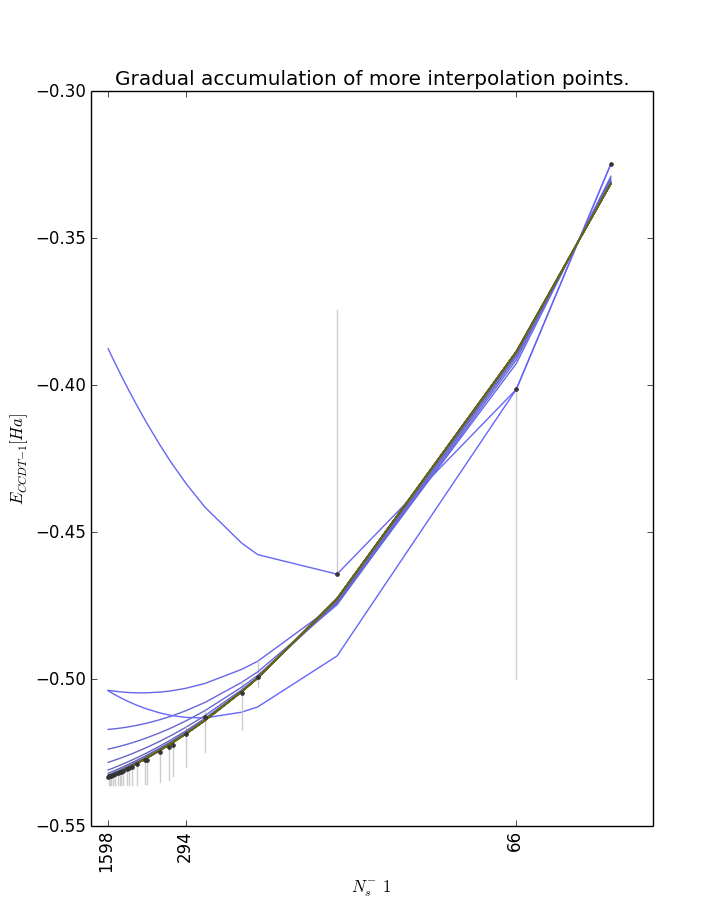
\includegraphics[width=0.8\textwidth]{accumulation}
    \caption{Gradual inclusion of more interpolation points (black dots) is assumed to bring us closer to the true thermodynamical limit estimate. The vertical lines indicates the estimated value for each interpolation point. }
    \label{fig:accumulation}
\end{figure}

The extrapolated energy is also plotted in the same diagram, beginning
with only the two leftmost data points resulting in the leftmost
thermodynamical limit estimate. As we move to the right, we also
accumulate more of the smaller basis sets, thereby also introducing
more finite-size effects.

\subsection{A note on obtaining the data}

While our CCSDT-1 implementation easily handles smaller basis sets on
a typical home computer, it quickly runs out of resources when we
scale up towards the basis set sizes usually presented in the
literature.

To obtain the data presented in Fig.~\ref{fig:extrapol}, we have run calculations
on the Abel Cluster of the university of Oslo, (see Ref. \cite{abel}). This cluster has nodes
which  offer up to one terabyte of memory. These are the so-called
\emph{hugemem} nodes.

To perform these calculations as efficiently as possible, we have
parallelized crucial parts of the code, such as the initialization of
the $\hat{T}_3$ amplitudes, as well as the iterative procedure. This
was achieved by the use of open MP \cite{openmp}. We also
eased the convergence criteria for these calculations, since the
iterations for systems of this size is time consuming. Given more time, it
is fully possible to obtain results with the same precision as we had
for the smaller basis sets.






\subsection{Results from the large basis extrapolation}

\begin{figure}[hbtp]
    \centering
    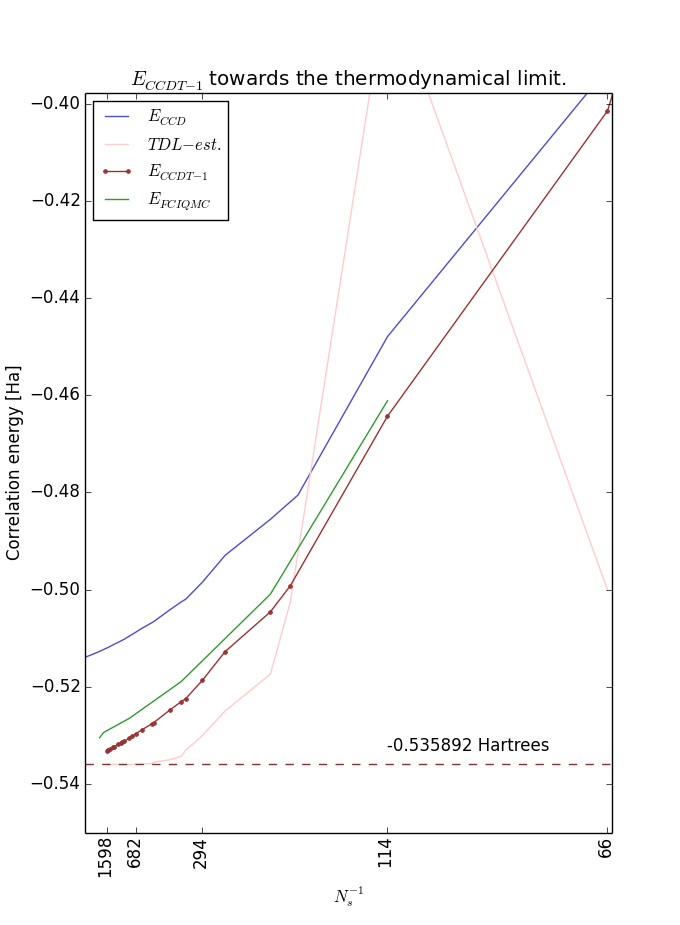
\includegraphics[width=0.8\textwidth]{ExtrapolationCCDT1final}
    \caption{Our CCDT-1 results compared to FCIQMC from Ref.~\cite{Shepherd2012} and CCD from Ref.~\cite{Baardsen2015}. The thermodynamical limit results are extrapolated using a polynomial fitting in $(N_s^{-1})^2$, and the inclusion of all data points results in the dotted horizontal line at $E_{CCDT-1}(N_s \rightarrow \infty) \approx -0.53589205$ Hartrees.}
    \label{fig:extrapol}
\end{figure}

The results from these calculations are shown in
Fig.~\ref{fig:extrapol}, while the actual energies are given in table
\ref{tab:extrap_large}. The number of basis functions in our data set
allows for a meaningful comparison with CCD and FCIQMC results in the
literature. Our calculations run up to $N_s = 1598$. Larger runs are needed for greater $N_s$
values. Such calculations will be performed in connection with our publication of the results. 


In table II of Ref.~\cite{Shepherd2012}, we find a comparable
estimate from FCIQMC caclulations using a \emph{single-point extrapolation} 
technique described in the same text. For $N_s=14$
and up to 1850 orbitals, Shepherd \emph{et al.} found a
thermodynamical limit estimate of $-0.5316(4)$ Hartrees, where the
number in the parenthesis represents the stochastic error. From table
\ref{tab:extrap_convergence}, we see that the CCDT-1 approach gives an estimate
approximately at just above $-0.536$ Hartrees. By comparison, using
the same technique on the CCD results from Ref.~\cite{Baardsen2015},
we obtain an estimate just above $-0.515$ Hartrees. (By correcting for
finite-size effects and incomplete basis error, Shepherd \emph{et al.}
obtained approximately $-0.546$ Hartrees from corresponding CCSD
calculations in Ref.~\cite{Shepherd2013}.)

In Ref.~\cite{Shepherd2013}, the authors were able to perform calculations
using CCD(T) for HEG systems of up to 200 particles. To overcome the
computational costs, they approximated these contributions in a way
that did not alter its qualitative behavior.  This approximation is
referred to as CCSD(scT). By using 700 to 1600 orbitals, they then
estimated the ground state energy to be approximately $-0.56$
Hartrees\footnote{Number obtained by visual inspection of Fig. 4 in
  Ref.~\cite{Shepherd2013}} for 14 electrons at $r_s = 1.0$


\begin{table}[hbpt]
\caption{Ground state energies from the CCDT-1 approach for $r_s = 1.0$}
\begin{center}
\begin{threeparttable}
\begin{tabular}{l l l}
    \toprule
    $N_s$ & $E_{CCDT-1}$ & $\Delta e_{f.i.}$ \\ \hline
54  & -0.3247616709272834  \\
66   &-0.4014439489508850  \\
114  &-0.4642919485466862 \\
168  &-0.4992170228805105 \\
186  &-0.5045720211973277 \\
246  &-0.5127494951081482 \\
294  &-0.5186916762333957 \\
342 & -0.5224209034109932 \\
358 & -0.5230371543102510 \\ \hline
406  &-0.52477086       &   4.83611717e-09 \\
502  &-0.52738302       &   5.08323494e-09\\
514 & -0.52759733         &  5.0938509e-09\\
610 & -0.52890112        &  5.18983734e-09 \\    
682 & -0.52973516        &  -9.0516229e-09  \\   
730 & -0.53016462          & 5.27640609e-09\\     
778 & -0.53055221        &  5.29870681e-09 \\    
874 & -0.53121663        &  5.33532052e-09 \\    
922 & -0.53145774        &  5.34856293e-09 \\   
970 & -0.53165927        &  5.35778177e-09 \\    
1030 &-0.53186170       &   5.36616518e-09\\     
1174 &-0.53231755        &  5.38305334e-09\\     
1238 &-0.53249388        &  5.3889998e-09  \\    
1382 &-0.53280698        &  5.3976934e-09  \\   
1478 &-0.53300407        &  5.40233591e-09\\     
1502&  -0.533038         &    5.40305467e-09  \\
1598 &-0.53317370        &  5.40562695e-09\\   
\bottomrule
\end{tabular}
\begin{tablenotes}
Results from computations on the so-called "hugemem" nodes on the Abel
cluster in the lower part of the table is separated by a horizontal
line from those obtained at an ordinary office computer. The precision
is decreased for these calculations to reduce the computation time,
but it given enough time (at most a couple of days) the precision may
be easily improved. The rightmost column shows deviation between the
two final iterations in the CCDT-1 and reflect our convergence
criteria.
\end{tablenotes}
\end{threeparttable}
\end{center}
\label{tab:extrap_large}
\end{table}

\begin{table}[h]
\caption{Convergence in the thermodynamical limit estimate.}
\begin{center}
\begin{threeparttable}
\begin{tabular}{l l l}
    \toprule
$N_s$ & Estimated energy \\ \hline
114&-0.500074170875 \\
168&-0.37448232\\
186&-0.50261060\\
246& -0.51739203\\
394&-0.52495653\\
342&-0.53004505\\
358&-0.53303659\\
406&-0.53430978\\
502&-0.53501392\\
514&-0.53551920\\
610&-0.53579986\\
682&-0.53590259\\
730&-0.53596398\\
778&-0.53599564\\
874&-0.53601389\\
922&-0.53602668\\
970&-0.53602951\\
1030&-0.53602389\\
1174&-0.53600828\\
1238&-0.53598359\\
1382&-0.53596086\\
1478&-0.53593480\\
1502&-0.53591225\\
1598&-0.53589205\\
\bottomrule
\end{tabular}
\begin{tablenotes}
Estimates of the thermodynamical limit ground state energy from CCDT-1 results on the homogeneous electron gas in 3D . We ignore finite-size effects and use the method visualized in Fig.\ref{fig:accumulation}. 
\end{tablenotes}
\end{threeparttable}
\end{center}
\label{tab:extrap_convergence}
\end{table}

\FloatBarrier
\section{Contributions from diagrams}

Introducing more diagrams in our calculations may have an effect on
the energy. Some diagrams may add to the energy, others may subtract,
and yet some may have no visible effect at all. Complicated couplings
of the diagrams may make it hard to unambiguously decide their proper role before having run the calculations.

A qualitative study of how each diagram contributes to the calculation
may yield some insights into which kind of excitations are important
in the system and which are not.

We begin by investigating how the gradual inclusion of the linear
$\hat{T}_3$ diagrams as well as the two extra diagrams in the
$\hat{T}_2$ amplitude due to the triple excitations affects the energy
up to the CCDT-1 equations. The results of this gradual inclusion is
shown for a range of $r_s$ values and $N_s = 54$ in
Fig. \ref{fig:ccdt1_sweep_corr}, while the deviation of these results
with the corresponding CCDT calculation is shown in
Fig. \ref{fig:ccdt1_sweep_dev}. Obviously,
Fig.\ref{fig:ccdt1_sweep_corr} is not that informative, since
contributions are tightly packed and hard to distinguish. Since we are
only after the contributions from each diagrams, we may therefore omit
such plots for the rest of the diagrams, as these will be even more
tightly packed. The full numerical results are provided in tables
\ref{tab:ccd_to_ccdt1_1} to \ref{tab:ccdt3_to_ccdt_3}.\footnote{These
  results may come in handy for those who wish to reproduce our
  results or in debug processes for similar codes. Please remember
  that these results have not been benchmarked against other calculations.}


\begin{figure}[!htb]
  \centering
  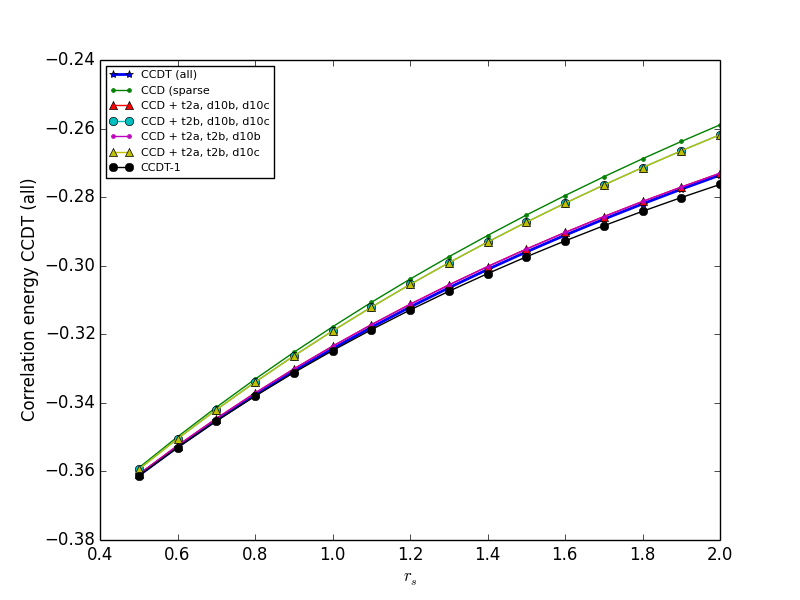
\includegraphics[width=230pt]{ccdt1_sweep_corr}
  \caption{Correlation energies in Hartrees for various inclusions of diagrams leading up to the CCDT-1 equation.}
\label{fig:ccdt1_sweep_corr}
\end{figure}



In Fig. \ref{fig:ccdt3_sweep_dev} we proceed by including even more
diagrams in the CCDT1 equation, until we have the CCDT2 equations with
contributions from all diagrams quadratic in $\hat{T}_2$. We then
finally inspect individually contributions from each of the "mixed"
$t2t3$ terms in Fig. \ref{fig:ccdt4_sweep_dev}. Note the notation for the mixed terms.

It is clear from all these results that most of the differences in the
various approximations diverge from the CCDT correlation energy as we
leave the high density regime where $r_s \leq 1.5$. One exception is
the combinations containing both $T_{2a}$ and $D_{10b}$ in
Fig. \ref{fig:ccdt1_sweep_dev}. The calculations with these
contributions overlaps almost perfectly above the CCDT
calculation in a quadratic shape, and indicate that it will cross the
CCDT correlation energy at some point. For $r_s = 2.0$, these
calculations are even closer to the CCDT energy than the complete
CCDT-1.

\begin{figure}[!htb]
\minipage{.5\textwidth}
  \centering
  \includegraphics[width=230pt]{ccdt1_sweep_dev}
  \caption{Deviations in Hartrees for the correlation energies from various truncations leading up to the CCDT-1 equation.}\label{fig:ccdt1_sweep_dev}
\endminipage\hfill
\minipage{.5\textwidth}
  \centering
  \includegraphics[width=230pt]{ccdt2_sweep_dev}
  \caption{Deviations in Hartrees for the correlation energies from various truncations leading up to the CCDT-2 equation.}\label{fig:ccdt2_sweep_dev}
\endminipage\hfill
\minipage{.5\textwidth}
\endminipage\hfill
\end{figure}

Generally, the deviations from the CCDT calculation decrease with
roughly a factor of $10^{-1}$ between CCD, CCDT1. CCDT2 and CCDT, as
may be seen by reading off the y-axes of the figures in question.

In the stage beginning with CCDT-1 and ending with CCDT-2 in
Fig. \ref{fig:ccdt2_sweep_dev}, we may clearly see the role of  the $(t2t2)_b$
term that adds in most of the CCDT-2 correlations.

From CCDT-2 to the inclusion of terms linear in $\hat{T}_3$, we see
that all diagrams contribute significantly, but that $(t3)_a$ is
responsible for most of additional correlation energy, while $(t3)_b$ has the least
impact.

\begin{figure}[!htb]
\minipage{.5\textwidth}
  \centering
  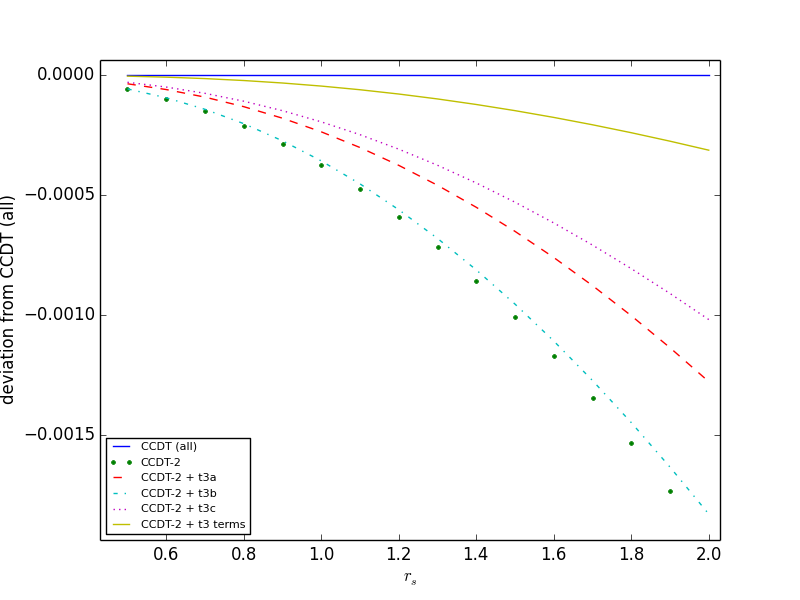
\includegraphics[width=230pt]{ccdt3_sweep_dev}
  \caption{Deviations in Hartrees for the correlation energies from various truncations beyond the CCDT-2 equation.}\label{fig:ccdt3_sweep_dev}
\endminipage\hfill
\minipage{.5\textwidth}
  \centering
  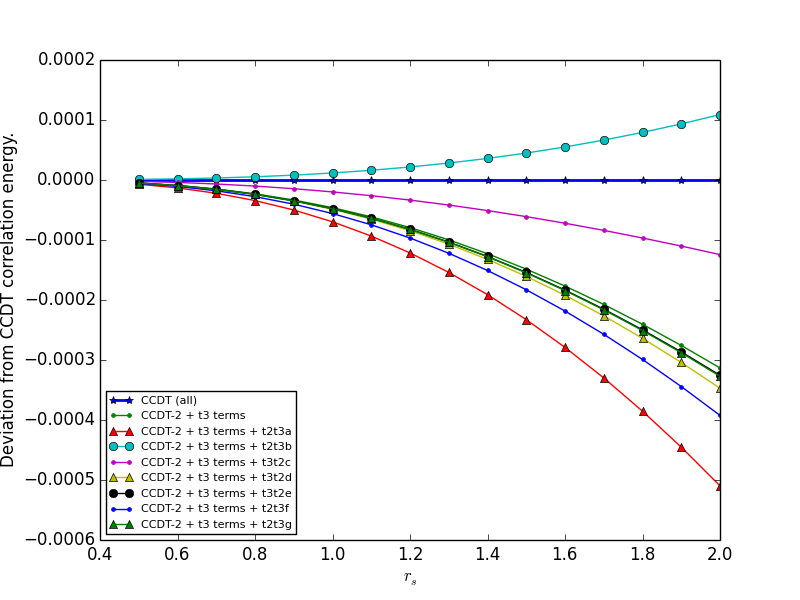
\includegraphics[width=230pt]{ccdt4_sweep_dev}
  \caption{Deviations in Hartrees for the correlation energies from including "mixed" terms in the $\hat{T}_3$ amplitude leading up to the CCDT equation.}
\label{fig:ccdt4_sweep}
\endminipage\hfill
\end{figure}

In the final stage, from CCDT-2 with linear $\hat{T}_3$ terms, ending
with CCDT, it is clear that the diagrams with the largest
contributions are $(t2t3)_b$ and $(t2t3)_c$, while these two are also
the only ones increasing the energy towards the full CCDT results. Is is also
worth noting that the diagram $(t2t3)_b$ also brings us above the CCSDT
energy, and thus closer to the true correlation energy given that
these results are comparable to the ones for $N_s = 114$.

The significance - if any - of these results are unclear to the
author, but the clear improvement from including only the diagrams
$T_{2a}$ and $d_{10b}$ does suggest that more numerical experiments with this
truncation are needed. Including only these diagrams could provide the means of
reducing the computational cost, as well as an improvement upon the CCDT-1
truncation outside the high density domain.











\FloatBarrier

\begin{table}[hbtp]
\caption{From CCD to CCDT1 (a)}
\begin{center}
\begin{threeparttable}
\begin{tabular}{l l l l l}
    \toprule
$r_s$ & CCDT (all) & CCD (sparse) & CCD+all t2t2 , $d_{10b}$, $d_{10c}$ & CCD+$t_{2a}$, $d_{10b}$, $d_{10c}$  \\ \hline
0.5 & -0.361182136242 & -0.358965573995 & -0.358937799509 & -0.360848662897   \\
0.6 & -0.35289477153 & -0.349913298941 & -0.349869014363 & -0.352467423986   \\
0.7 & -0.345095172951 & -0.34129880764 & -0.341233775603 & -0.344578165852   \\
0.8 & -0.337741036665 & -0.33309549971 & -0.333005531117 & -0.337141804947  \\
0.9 & -0.330794429481 & -0.325278123609 & -0.325159145375 & -0.330122838461   \\
1.0 & -0.324221302444 & -0.317822843689 & -0.317670940833 & -0.323489024517   \\
1.1 & -0.317991054686 & -0.310707258113 & -0.310518697541 & -0.317211078584  \\
1.2 & -0.312076145029 & -0.30391038201 & -0.303681623395 & -0.311262390387   \\
1.3 & -0.306451747765 & -0.297412606757 & -0.297140304484 & -0.305618763253   \\
1.4 & -0.301095448541 & -0.291195643538 & -0.290876642595 & -0.300258176233   \\
1.5 & -0.295986976242 & -0.285242457229 & -0.28487378513 & -0.295160568459   \\
1.6 & -0.291107966848 & -0.279537195014 & -0.279116051241 & -0.290307644542   \\
1.7 & -0.286441755584 & -0.27406511291 & -0.273588856927 & -0.285682699556   \\
1.8 & -0.281973193938 & -0.268812502441 & -0.268278641007 & -0.281270462005   \\
1.9 & -0.277688488513 & -0.263766619014 & -0.263172793299 & -0.277056953128   \\
2.0 & -0.273575059003 & -0.258915613005 & -0.258259585841 & -0.273029360975   \\
\bottomrule
\end{tabular}
\begin{tablenotes}
\end{tablenotes}
\end{threeparttable}
\end{center}
\label{tab:ccd_to_ccdt1_1}
\end{table}

\begin{table}[hbtp]
\caption{From CCD to CCDT1 (b)}
\begin{center}
\begin{threeparttable}
\begin{tabular}{l l l l l}
    \toprule
$r_s$ & CCD+$t_{2b}$, $d{10b}$, $d_{10c}$ & CCD+$t_{2a}$, $t_{2b}$, $d_{10b}$ & CCD+$t_{2a}$, $t_{2b}$, $d_{10c}$ & CCDT-1  \\ \hline
0.5 & -0.359382812741 & -0.360848610871 & -0.35938286414 & -0.361271280331   \\
0.6 & -0.350475868693 & -0.352467326244 & -0.350475964803 & -0.353040097402   \\
0.7 & -0.342016839697 & -0.344578001572 & -0.342017000386 & -0.345313192843   \\
0.8 & -0.333976230676 & -0.337141550367 & -0.333976478267 & -0.338048918278   \\
0.9 & -0.326326455022 & -0.330122467573 & -0.326326813525 & -0.331209710045   \\
1.0 & -0.319041801529 & -0.323488509766 & -0.319042295892 & -0.324761670927   \\
1.1 & -0.312098369047 & -0.317210391538 & -0.312099024469 & -0.318674187521   \\
1.2 & -0.30547398076 & -0.31126150236 & -0.305474822082 & -0.312919583715   \\
1.3 & -0.299148086706 & -0.30561764586 & -0.2991491379 & -0.307472809107   \\
1.4 & -0.29310166071 & -0.30025680189 & -0.293102944449 & -0.302311160242   \\
1.5 & -0.287317096026 & -0.295158910812 & -0.287318633349 & -0.29741403209   \\
1.6 & -0.281778102658 & -0.290305678835 & -0.281779912717 & -0.292762696991   \\
1.7 & -0.276469608293 & -0.285680402945 & -0.276471708165 & -0.288340108337   \\
1.8 & -0.27137766407 & -0.281267813814 & -0.27138006864 & -0.284130726343   \\
1.9 & -0.266489355882 & -0.277053935064 & -0.266492077776 & -0.280120363495   \\
2.0 & -0.261792721537 & -0.273025957299 & -0.261795771106 & -0.276296047416   \\
\bottomrule
\end{tabular}
\begin{tablenotes}
\end{tablenotes}
\end{threeparttable}
\end{center}
\label{tab:ccd_to_ccdt1_2}
\end{table}

\begin{table}[hbtp]
\caption{From CCDT1 to CCDT2 (a)}
\begin{center}
\begin{threeparttable}
\begin{tabular}{l l l l}
    \toprule
$r_s$ & CCDT(all) & CCDT-1 & CCDT-1+$(t2t2)_b$  \\ \hline
0.5 & -0.361182136242 & -0.361271280331 & -0.361241081392   \\
0.6 & -0.35289477153 & -0.353040097402 & -0.352991511388   \\
0.7 & -0.345095172951 & -0.345313192843 & -0.345241188004   \\
0.8 & -0.337741036665 & -0.338048918278 & -0.33794837969   \\
0.9 & -0.330794429481 & -0.331209710045 & -0.331075519112   \\
1.0 & -0.324221302444 & -0.324761670927 & -0.324588760945   \\
1.1 & -0.317991054686 & -0.318674187521 & -0.318457581714   \\
1.2 & -0.312076145029 & -0.312919583715 & -0.312654420478   \\
1.3 & -0.306451747765 & -0.307472809107 & -0.307154357932   \\
1.4 & -0.301095448541 & -0.302311160242 & -0.301934830914   \\
1.5 & -0.295986976242 & -0.29741403209 & -0.296975379025   \\
1.6 & -0.291107966848 & -0.292762696991 & -0.292257420127   \\
1.7 & -0.286441755584 & -0.288340108337 & -0.287764051589   \\
1.8 & -0.281973193938 & -0.284130726343 & -0.283479874385   \\
1.9 & -0.277688488513 & -0.280120363495 & -0.279390837409   \\
2.0 & -0.273575059003 & -0.276296047416 & -0.275484099609   \\
\bottomrule
\end{tabular}
\begin{tablenotes}
\end{tablenotes}
\end{threeparttable}
\end{center}
\label{tab:ccdt1_to_ccdt2_1}
\end{table}


\begin{table}[hbtp]
\caption{From CCDT1 to CCDT2 (b)}
\begin{center}
\begin{threeparttable}
\begin{tabular}{l l l l}
    \toprule
$r_s$ & CCDT-1+$(t2t2)_c$ & CCDT-1 + $(t2t2)_d$ & CCDT-2  \\ \hline
0.5 & -0.361272932544 & -0.361270990289 & -0.361242443   \\
0.6 & -0.353042798434 & -0.353039597895 & -0.352993711412   \\
0.7 & -0.345317255471 & -0.345312404144 & -0.345244458542   \\
0.8 & -0.338054668921 & -0.338047749984 & -0.337952955242   \\
0.9 & -0.33121748294 & -0.331208062146 & -0.331081631683   \\
1.0 & -0.324771803463 & -0.324759434901 & -0.324596636327   \\
1.1 & -0.318687016504 & -0.318671247419 & -0.318467436695   \\
1.2 & -0.312935442374 & -0.31291581723 & -0.312666460793   \\
1.3 & -0.307492024708 & -0.30746808862 & -0.307168776809   \\
1.4 & -0.302334052183 & -0.302305353836 & -0.301951808081   \\
1.5 & -0.297440910392 & -0.29740700453 & -0.296995080102   \\
1.6 & -0.292793861102 & -0.29275431068 & -0.292279996315   \\
1.7 & -0.2883758462 & -0.288330224228 & -0.2877896396   \\
1.8 & -0.28417131367 & -0.284119204837 & -0.283508596572   \\
1.9 & -0.280166063215 & -0.2801070653 & -0.279422802045   \\
2.0 & -0.276347109259 & -0.276280834387 & -0.275519401298   \\
\bottomrule
\end{tabular}
\begin{tablenotes}
\end{tablenotes}
\end{threeparttable}
\end{center}
\label{tab:ccd1_to_ccdt2_2}
\end{table}

\begin{table}[hbtp]
\caption{From CCDT2 to CCDT2 + linear t3 (a)}
\begin{center}
\begin{threeparttable}
\begin{tabular}{l l l l}
    \toprule
$r_s$ & CCDT & CCDT-2 & CCDT-2 +$(t3)_a$  \\ \hline
0.5 & -0.361182136242 & -0.361242443 & -0.361218738719   \\
0.6 & -0.35289477153 & -0.352993711412 & -0.352955389336   \\
0.7 & -0.345095172951 & -0.345244458542 & -0.345187410081   \\
0.8 & -0.337741036665 & -0.337952955242 & -0.337872969247   \\
0.9 & -0.330794429481 & -0.331081631683 & -0.330974462634   \\
1.0 & -0.324221302444 & -0.324596636327 & -0.324458053866   \\
1.1 & -0.317991054686 & -0.318467436695 & -0.318293261114  \\
1.2 & -0.312076145029 & -0.312666460793 & -0.312452587945   \\
1.3 & -0.306451747765 & -0.307168776809 & -0.306911195085  \\
1.4 & -0.301095448541 & -0.301951808081 & -0.301646609441   \\
1.5 & -0.295986976242 & -0.296995080102 & -0.296638466677   \\
1.6 & -0.291107966848 & -0.292279996315 & -0.291868283709   \\
1.7 & -0.286441755584 & -0.2877896396 & -0.287319257769  \\
1.8 & -0.281973193938 & -0.283508596572 & -0.282976088915   \\
1.9 & -0.277688488513 & -0.279422802045 & -0.278824823213   \\
2.0 & -0.273575059003 & -0.275519401298 & -0.274852714074   \\
\bottomrule
\end{tabular}
\begin{tablenotes}
\end{tablenotes}
\end{threeparttable}
\end{center}
\label{tab:ccd2_to_ccdt3_1}
\end{table}

\begin{table}[hbtp]
\caption{From CCDT2 to CCDT2 + linear t3 (b)}
\begin{center}
\begin{threeparttable}
\begin{tabular}{l l l l}
    \toprule
$r_s$ & CCDT-2 + t3b & CCDT-2 + $(t3)_c$ & CCDT-2 + t3(all)  \\ \hline
0.5 & -0.361240074436 & -0.361212496588 & -0.361186968791   \\
0.6 & -0.352989680206 & -0.352945032659 & -0.352903754956   \\
0.7 & -0.345238159145 & -0.345171587896 & -0.345110139593   \\
0.8 & -0.337943708706 & -0.337850204441 & -0.337764065954   \\
0.9 & -0.331068693447 & -0.33094316437 & -0.330827795998   \\
1.0 & -0.324579203596 & -0.324416526415 & -0.324267427027   \\
1.1 & -0.318444655364 & -0.318239709672 & -0.318052460081   \\
1.2 & -0.312637431899 & -0.312385121921 & -0.312155416584   \\
1.3 & -0.307132562511 & -0.306827829204 & -0.306551499031   \\
1.4 & -0.301907437187 & -0.30154526299 & -0.301218291375   \\
1.5 & -0.296941553166 & -0.296516961116 & -0.296135494817   \\
1.6 & -0.292216290327 & -0.291724338872 & -0.291284694974   \\
1.7 & -0.287714712303 & -0.2871504868 & -0.286649156719   \\
1.8 & -0.283421390437 & -0.282779992098 & -0.282213643357   \\
1.9 & -0.279322247926 & -0.278598780801 & -0.277964257128   \\
2.0 & -0.27540442181 & -0.274593978214 & -0.27388829842   \\
\bottomrule
\end{tabular}
\begin{tablenotes}
\end{tablenotes}
\end{threeparttable}
\end{center}
\label{tab:ccd2_to_ccdt3_2}
\end{table}


\begin{table}[hbtp]
\caption{From CCDT2 + linear t3 to CCDT (a)}
\begin{center}
\begin{threeparttable}
\begin{tabular}{l l l l}
    \toprule
$r_s$ & CCDT & CCDT-2 + t3(all) & CCDT-2 + t3(all) + $(t2t3)_a$  \\ \hline
0.5 & -0.361182136242 & -0.361186968791 & -0.361189161494   \\
0.6 & -0.35289477153 & -0.352903754956 & -0.352907932372   \\
0.7 & -0.345095172951 & -0.345110139593 & -0.345117267621   \\
0.8 & -0.337741036665 & -0.337764065954 & -0.337775292461  \\
0.9 & -0.330794429481 & -0.330827795998 & -0.33084443613   \\
1.0 & -0.324221302444 & -0.324267427027 & -0.324290947458   \\
1.1 & -0.317991054686 & -0.318052460081 & -0.318084463335   \\
1.2 & -0.312076145029 & -0.312155416584 & -0.31219762608   \\
1.3 & -0.306451747765 & -0.306551499031 & -0.306605745257   \\
1.4 & -0.301095448541 & -0.301218291375 & -0.301286499351   \\
1.5 & -0.295986976242 & -0.296135494817 & -0.296219672924   \\
1.6 & -0.291107966848 & -0.291284694974 & -0.291386925122   \\
1.7 & -0.286441755584 & -0.286649156719 & -0.286771585795   \\
1.8 & -0.281973193938 & -0.282213643357 & -0.282358475852   \\
1.9 & -0.277688488513 & -0.277964257128 & -0.278133748843   \\
2.0 & -0.273575059003 & -0.27388829842 & -0.27408475114   \\
\bottomrule
\end{tabular}
\begin{tablenotes}
\end{tablenotes}
\end{threeparttable}
\end{center}
\label{tab:ccdt3_to_ccdt_1}
\end{table}

\begin{table}[hbtp]
\caption{From CCDT2 + linear t3 to CCDT (b)}
\begin{center}
\begin{threeparttable}
\begin{tabular}{l l l l}
    \toprule
$r_s$ & CCDT-2 + t3(all)+$(t2t3)_b$ & CCDT-2 + t3(all)+$(t3t2)_c$ & CCDT-2 +t3(all)+$(t3t2)_d$  \\ \hline
0.5 & -0.361181173957 & -0.361184340036 & -0.361187127038   \\
0.6 & -0.352892878689 & -0.352898818243 & -0.352904091207   \\
0.7 & -0.345091851048 & -0.345101835074 & -0.345110770555   \\
0.8 & -0.337735673415 & -0.337751170412 & -0.337765146693   \\
0.9 & -0.330786303973 & -0.330808950068 & -0.330829522494   \\
1.0 & -0.324209592489 & -0.324241162451 & -0.324270037743   \\
1.1 & -0.317974845376 & -0.318017225821 & -0.318056236736   \\
1.2 & -0.312054437757 & -0.312109603165 & -0.312160684269   \\
1.3 & -0.306423469119 & -0.306493460869 & -0.306558625822   \\
1.4 & -0.30105945867 & -0.301146367031 & -0.301227687558   \\
1.5 & -0.295942076381 & -0.296048025283 & -0.296147611826   \\
1.6 & -0.291052905834 & -0.291180040147 & -0.291300024139   \\
1.7 & -0.286375235231 & -0.286525710259 & -0.286668227882   \\
1.8 & -0.281893873224 & -0.282069846146 & -0.282237023418   \\
1.9 & -0.277594986573 & -0.27779860954 & -0.277992548569   \\
2.0 & -0.273465956943 & -0.273699371593 & -0.273922137838   \\
\bottomrule
\end{tabular}
\begin{tablenotes}
\end{tablenotes}
\end{threeparttable}
\end{center}
\label{tab:ccdt3_to_ccdt_2}
\end{table}

\begin{table}[hbtp]
\caption{From CCDT2 + linear t3 to CCDT (c)}
\begin{center}
\begin{threeparttable}
\begin{tabular}{l l l l}
    \toprule
$r_s$ & CCDT-2 + t3(all)+$(t3t2)_e$ & CCDT-2 + t3(all)+$(t2t3)_f$ & CCDT-2 + t3(all)+$(t2t3)_g$  \\ \hline
0.5 & -0.361187132882 & -0.361187901826 & -0.361187148223   \\
0.6 & -0.352904063306 & -0.352905522504 & -0.352904092948   \\
0.7 & -0.345110658791 & -0.345113140129 & -0.345110710161   \\
0.8 & -0.337764873187 & -0.337768769556 & -0.337764955452   \\
0.9 & -0.330828977512 & -0.330834737646 & -0.330829101587   \\
1.0 & -0.324269076573 & -0.324277199626 & -0.324269255115   \\
1.1 & -0.318054677444 & -0.318065707615 & -0.318054924807   \\
1.2 & -0.312158306205 & -0.312172827611 & -0.312158638377   \\
1.3 & -0.306555168756 & -0.306573800645 & -0.306555603257   \\
1.4 & -0.30122285132 & -0.301246243665 & -0.301223407072   \\
1.5 & -0.296141056346 & -0.296169885828 & -0.296141753505   \\
1.6 & -0.291291369789 & -0.291326336145 & -0.291292229537   \\
1.7 & -0.286657056042 & -0.286698878762 & -0.286658100338   \\
1.8 & -0.282222877189 & -0.282272292533 & -0.282224128479   \\
1.9 & -0.277974933588 & -0.278032691874 & -0.277976414461   \\
2.0 & -0.273900523131 & -0.273967386287 & -0.273902255934   \\
\bottomrule
\end{tabular}
\begin{tablenotes}
\end{tablenotes}
\end{threeparttable}
\end{center}
\label{tab:ccdt3_to_ccdt_3}
\end{table}

\FloatBarrier

\section{Benchmarking}

Performance benchmarks are provided for both our implementations in
Figs. \ref{fig:it2}, \ref{fig:it}, \ref{fig:ini2}, \ref{fig:inia} and
\ref{fig:inib}. Note that not all parts of our two algorithms have implemented OpenMP
\cite{openmp} in a consisted way, essentially due to lack of time. We
have obtained some performance benchmarks from Baardsen (in
Ref. \cite{Baardsen2015}) that clearly indicate that his CCD
implementation outperforms our own. For the largest basis set
benchmarked in Figs. \ref{fig:it2} and \ref{fig:ini2}, Baardsen
measured only 5 seconds CPU time in total, whereas the initialization
time in our implementation is approximately 6 second and each
iteration is performed in approximately 0.4 seconds.

\begin{figure}[!htb]
  \centering
  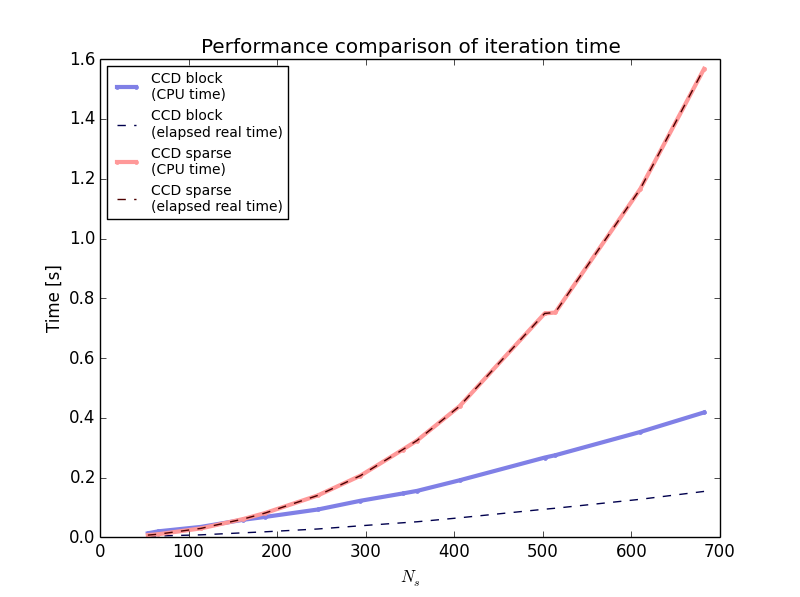
\includegraphics[width=230pt]{iterations2}
  \caption{Elapsed real time and CPU time for the CCD iterations.}
\label{fig:it2}
\end{figure}

\begin{figure}[!htb]
  \centering
  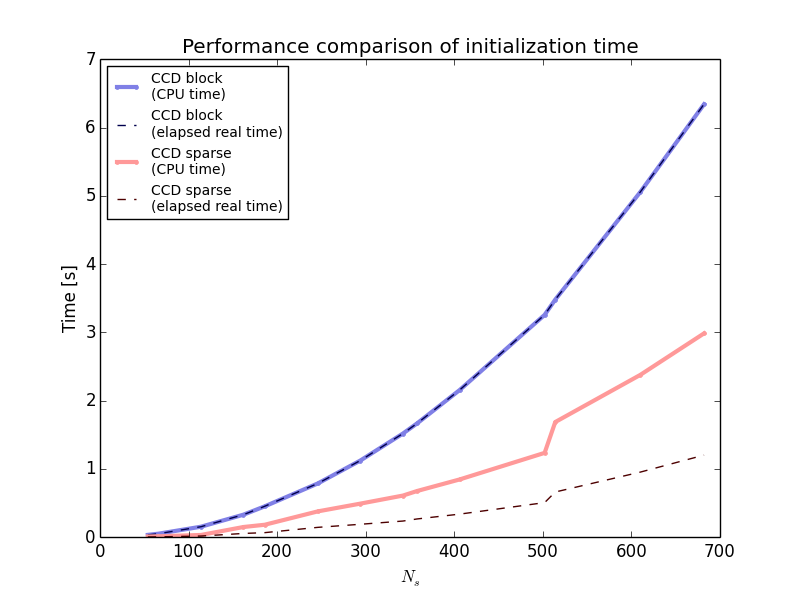
\includegraphics[width=230pt]{initializations_2}
  \caption{Elapsed real time and CPU time for the CCD iterations.}
\label{fig:ini2}
\end{figure}

Some of this discrepancy may be explained by the fact that the
compiler provided by Intel used by Baardsen is known to give better
performance than the GNU compiler used by us (see
Ref. \cite{abel_drift}), but since our main focus has been to
efficiently optimize the bottlenecks in our CCDT implementations, we
have neglected such bottlenecks in the plain CCD implementation. The
performance issues that arise from inclusion of the triple amplitudes
overshadows the CCD challenges by far, so any improvement in the CCD
implementation would probably not give any significant boost in performance to our
CCDT implementation. Other explanations could be related to differences between
Fortran and C++, such as the many compiler challenges posed by the
object orientation in C++.

When comparing the CCDT-1 imlementations in Figs.\ref{fig:it},
\ref{fig:inia} and \ref{fig:inib}, it is interesting to note the very
large deviation in the initialization time between the two. The reason
for this is that the sparse solver does not require any mapping of
channels in the diagrams. As we discussed in detail in chapter
\ref{Chapter7}, we may then avoid any sorting of large arrays in the
initialization, although initializing the sparse matrices will require
some sorting at a later stage. Still, the block implementation
outperforms the sparse by far in the CCD iterations, since these
actually requires both sorting and traversing of lists, while the
block implementation benefits greatly from the BLAS3 optimization of
the dense matrix-matrix multiplication.


\begin{figure}[!htb]
  \centering
  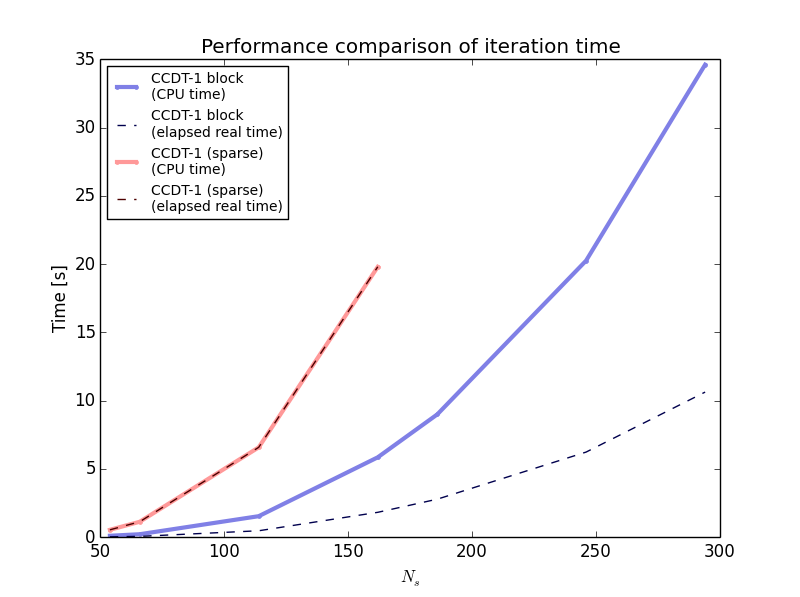
\includegraphics[width=230pt]{iterations}
  \caption{Elapsed real time and CPU time for the CCD-1 iterations.}
\label{fig:it}
\end{figure}

\begin{figure}[!htb]
  \centering
  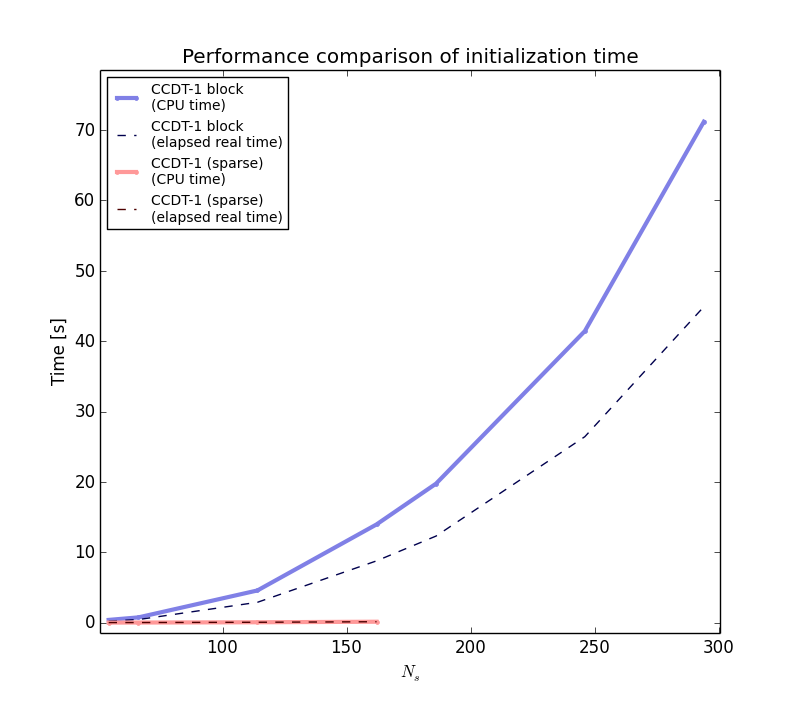
\includegraphics[width=230pt]{initializations_a}
  \caption{Elapsed real time and CPU time for the CCD-1 initializations.}
\label{fig:inia}
\end{figure}

\begin{figure}[!htb]
  \centering
  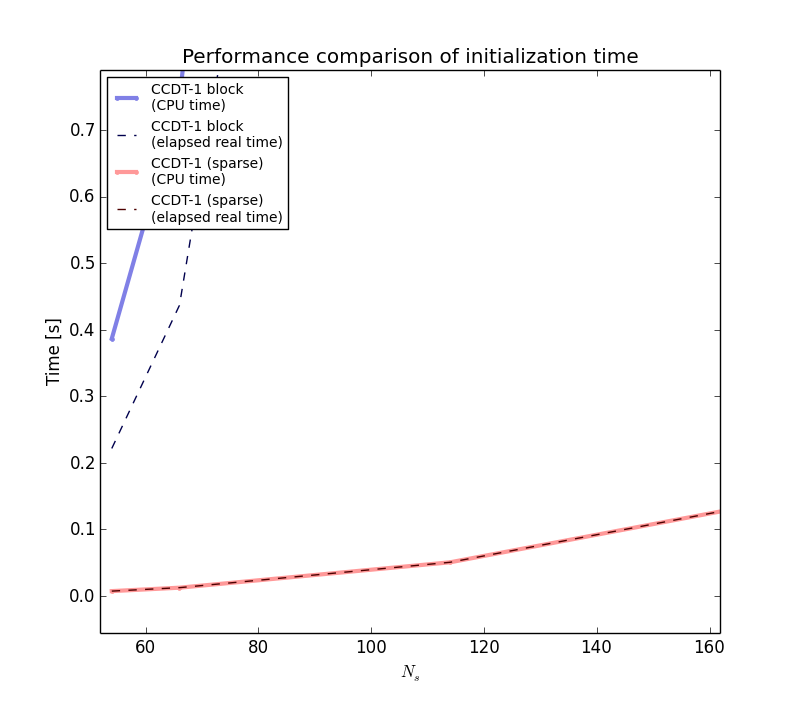
\includegraphics[width=230pt]{initializations_b}
  \caption{Elapsed real time and CPU time for the CCD-1 initializations. (Zoomed)}
\label{fig:inib}
\end{figure}


\begin{table}[hbtp]
\caption{Number of nonzero entries in the $\hat{T}_3$ amplitude}
\begin{center}
\begin{threeparttable}
\begin{tabular}{l l l}
    \toprule
$N_s$ & $N_{nonzeros}$ \\ \hline 
54 & 247777 \\
66 & 503209 \\ 
114 & 2745529 \\
162 & 7813177 \\
186 & 11025937 \\
246 & 21651901 \\
294 & 34037605 \\
\bottomrule
\end{tabular}
\begin{tablenotes}
The table shows the length of the element vector in the $\hat{T}_3$ amplitude, indicating memory requirements as a function of basis size.
\end{tablenotes}
\end{threeparttable}
\end{center}
\label{tab:memscale}
\end{table}

Table \ref{tab:memscale} indicates the relation between the basis set
size and the memory requirements for the $\hat{T}_3$ amplitude. The right
column shows the number of nonzero elements in the $\hat{T}_3$
amplitude. For each such nonzero element, several associated values
are stored, providing us with a rough estimate of the memory usage of our CCDT-1
implementation. Multiplying this number with 8 for each
such associated data container and multiplying this number with the number of
bytes used for each stored value, gives us a rough estimate of the memory needed. All these data types in our
implementation use 64 bits by default.
This indicates a memory usage of approximately 2 GB
for the largest basis set in table \ref{tab:memscale}, which agrees
with observations made during runtime.\footnote{The author did not
  perform extensive studies of the memory usage, although we used
  Valgrind extensively in the debugging process. The qualitative observations
  mentioned here were obtained using the "top" command during runtime in
  Ubuntu.}

\section{Brief summary}
In summary, we have validated our CCD results against existing ones
from the scienfitic literature. Furthermore, two different algorithms
for computing triples correlations give to numerical precision the
same results.

Our results for triples correlations applied to the homogenoeus
electron gas show clearly that these correlations play an important
role, bringing our coupled cluster calculations close to the benchmark
results obtained with other {\em ab initio} methods like full
configuration interaction quantum Monte Carlo. We note that for larger
radii $r_s$, more complicated correlations may be needed. Our results
are however very encouraging, and applications of our codes and
software to systems like infinite nuclear matter may provide {\em ab initio} benchmarks calculations for the nuclear equation of state.

In the next and final chapter, we summarize our results and present perspectives for future studies as well.
